%-----------------------------------------------------------------------------
%
%               Template for sigplanconf LaTeX Class
%
% Name:         sigplanconf-template.tex
%
% Purpose:      A template for sigplanconf.cls, which is a LaTeX 2e class
%               file for SIGPLAN conference proceedings.
%
% Guide:        Refer to "Author's Guide to the ACM SIGPLAN Class,"
%               sigplanconf-guide.pdf
%
% Author:       Paul C. Anagnostopoulos
%               Windfall Software
%               978 371-2316
%               paul@windfall.com
%
% Created:      15 February 2005
%
%-----------------------------------------------------------------------------


\documentclass[numbers,numberedpars]{sigplanconf}

% The following \documentclass options may be useful:

% preprint      Remove this option only once the paper is in final form.
% 10pt          To set in 10-point type instead of 9-point.
% 11pt          To set in 11-point type instead of 9-point.
% numbers       To obtain numeric citation style instead of author/year.

\usepackage{amsmath}

\newcommand{\cL}{{\cal L}}

\usepackage{listings}
\usepackage{color}
\usepackage{textcomp}
\usepackage{graphicx}
\usepackage{stmaryrd}
\usepackage{caption}
\usepackage{mathtools}
\usepackage[lite,subscriptcorrection,slantedGreek,nofontinfo]{mtpro2}

\lstset{language=Scheme}
\definecolor{codegreen}{rgb}{0,0.6,0}
\definecolor{codegray}{rgb}{0.5,0.5,0.5}
\definecolor{backcolour}{rgb}{0.95,0.95,0.92}
 
%\bibliographystyle{abbrvnat}
%\setcitestyle{sorting=none}  %super,open={[},close={]}}

\begin{document}

\special{papersize=8.5in,11in}
\setlength{\pdfpageheight}{\paperheight}
\setlength{\pdfpagewidth}{\paperwidth}

\conferenceinfo{Scheme and Functional Programming Workshop}{September 18th, 2016, Nara, Japan}
\copyrightyear{2016}
%\copyrightdata{978-1-nnnn-nnnn-n/yy/mm}
%\copyrightdoi{nnnnnnn.nnnnnnn}

% Uncomment the publication rights you want to use.
%\publicationrights{transferred}
\publicationrights{licensed}     % this is the default
%\publicationrights{author-pays}

\titlebanner{This paper is a draft}        % These are ignored unless
\preprintfooter{short description of paper}   % 'preprint' option specified.

\title{Multi-purpose web framework design based on websocket over HTTP Gateway}
\subtitle{A case study on GNU Artanis}

\authorinfo{Mu Lei}
           {SZDIY Community}
           {mulei@gnu.org}

\maketitle

\begin{abstract}
  The traditional Internet communication is largely based on HTTP protocol, which provides hyperlinked, stateless exchange of information.
  Although HTTP is convenient and easy to understand, it's problematic for real-time data exchange. Websockets protocol is one of the ways
  to solve the problem. It reduces overhead and provides efficient, stateful communication between client and server \citep{6197172}.
  
  This paper introduces a web framework design in Scheme programming language, which takes advantage of websocket protocol to provide both
  convenience and efficiency. In addition to the expressiveness, Scheme provides powerful abstract ability to implement co-routines with
  {\it continuations} for the server core.

  One of the significant aims is to design a high performance generic server core with {\it delimited continuations}, and we'll show how it's
  useful for Internet of Things (IoT).
  
  GNU Artanis also provides useful modules for web programming, RESTful, web caching, templating, MVC, and a novel abstraction for relational
  mapping to operate databases. We'll give it a summary in the rest of the paper.
\end{abstract}

\category{D.3.3}{Programming Languages}{Language Constructs and Features}[Frameworks]

% general terms are not compulsory anymore,
% you may leave them out
\terms
Scheme, framework

\keywords
Scheme, web framework, websocket, delimited continuation, co-routine, generic server

\section{Introduction}

Web framework is a library for rapid prototyping web development, and usually provide CLI (Command Line Interface) or
GUI (Graphical User Interface) tools to generate code for reducing workload according to certain patterns specified by the developers.
In addition to using web specific language such as PHP, the older approach for web programming is CGI (Common Gateway Interface).
Although many people think CGI is outdated, it is simple to understand and easy to use.
It can yet be regarded as a practical way for web programming.

But the industry always requires more: a fast way for rapid prototyping, an approach for both productivity and reliability, clean and DRY
(Don't Repeat Yourself) for maintaining, high level abstract for hiding details, less coding, securities, etc.
Most of the modern web frameworks such as Ruby on Rails provides the tools necessary to produce a web application model,
which is the underlying program itself \citep{1597080}. 

This paper will use the term {\it HTTP Gateway} to indicate the unified connection management interfaces and verification methods of websocket
over HTTP. The {\it HTTP Gateway} is not a new concept, actually it's hidden in many server design. It is worth to discuss it explicitly,
for it is important to understand how GNU Artanis manages all the websocket connections. We'll mention it in \ref{HTTP Gateway}.

In addition, this paper will show a different way to implement concurrent server. It is different from the callback way used in C or Node.js.
The {\it continuations} commonly used to implement concurrent processes
\citep{Krishnamurthi2007}\citep{Hieb:1990:CC:99164.99178}\citep{Hieb:1994:SUB:184324.184330}.
It is proved that {\it continuations} could be the model for directly expressing concurrency in Scheme language \citep{shivers1997continuations}.
In this paper, we'll take GNU Artanis as a study case to indicate the same purpose. Moreover,
GNU Artanis uses GNU Guile which is a practical Scheme implementation which provides {\it delimited continuations} for better implementing co-routines.
In this paper, we'll show a new way with the feature named {\it delimited continuations}, which is better abstract than traditional {\it continuations}.
We'll discuss it in \ref{Delimited Continuations}.

The C10K (concurrent in 10,000) and C10M (concurrent in 10,000,000) problem has told us that the performance is not the only thing to concern
for high concurrent server, but also the scalability.  
The old method is to use select() or poll() has $O(n)$ complexity, which is the handicap to hold more connections \citep{lemon2001kqueue}.
The new method is kqueue()/epoll()/IOCP which has O(1) complexity to query available connection sockets. We'll take epoll() as an example to
discuss the scalability issue in \ref{Concurrency}.

Websockets is a protocol for two-way communication between client and server over TCP connection. The client is, in a broad sense,
unnecessary to be a web browser. One of the benefit of websocket is that the developers could take advantage of TLS used in HTTPS for
encryption. And another is that unified listening port for arbitrary services. We will discuss websocket in \ref{Websocket}.

Finally, we'll discuss some of the notable features of GNU Artanis in \ref{Some features in GNU Artanis}.

\section{Some background knowledge}

It is simplified to explain {\it continuations} and {\it delimited continuations} in continuation passing style (CPS), and we'll show how to
transfer their definition in semantics to Scheme code naturally for practical programming.

\subsection{First Class Continuations}

A {\it continuation} is ``the rest of the computation''. In Scheme, {\it continuation} is implemented as {\it first class continuation},
which is often referred to as {\it call/cc} standing for
{\it call-with-current-continuation}. It captures (reifies) the state of underlying machine state named the {\it current continuation}.
The captured {\it continuation} is also referred as {\it escape procedure} passed into the scope by the argument (as a function) of {\it call/cc}.
When the {\it escape procedure} is called within the context, the run-time discards the
{\it continuation} at the time point of the calling and throws the previous captured {\it continuation} back into the machine state.

The {\it continuations} captured by {\it call/cc} often implies {\it first class}, which means a continuation
could be passed and returned from functions, and stored in a data structure with indefinite extent.
For its ``lightweight fork ability for parallel histories'' avoiding to trap into the operating system kernel, it's widely considered
to be the ideal method to implement lightweight threads (co-routines/green threads), although it's also useful in many areas, such as
backtracking, exception handling, and control flow analysis, etc.


\begin{figure}[tbph]
  \raggedright
  \begin{align*}
    \shortintertext{ {\it variable}: }
    \llbracket{x}\rrbracket\rho \quad&=\quad \lambda{\kappa}.(\kappa \: (\rho \: x))
    \\
    \shortintertext{ {\it $\lambda$\textendash abstract}: }
    \llbracket{\lambda{x}.M}\rrbracket\rho \quad&=\quad
    \lambda{\kappa}.(\kappa\:\:\lambda{v\kappa'}.(\llbracket{M}\rrbracket\rho[x \mapsto v]\:\:\kappa'))
    \\
    \shortintertext{ {\it application}: }
    \llbracket{(M\:N)}\rrbracket\rho \quad&=\quad
    \lambda{\kappa}.(\llbracket{M}\rrbracket\rho\:\:\lambda{m}.(\llbracket{N}\rrbracket\rho\:\:\lambda{n}.((m\:n)\:\kappa)))
  \end{align*}
  \caption{Continuation Semantics in spirit of CPS
    \citep{Danvy92representingcontrol:}\citep{Gasbichler:2002:FSC:581478.581504}.}
    \label{fig:cont_sema}
\end{figure}

The $\llbracket{...}\rrbracket\rho$ as a compound form means a simplified one-pass CPS transformation with an environment $\rho$
which maps variables to values. This specific CPS transformation should be constrained by two conditions:
$(1)$ Shouldn't introduce any administrative redex (the reducible expression operated by a continuation capturing lambda);
$(2)$ Wouldn't reduce the source term. And $E[...\mapsto...]$ means capture-avoiding substitution in expression $E$.
The term $(E_1\:E_2)$ represents the application of a function $E_1$ to an input $E_2$. The $\kappa$
is {\it continuation} which has the type that a function from values to values. In spirit of CPS,
the $\lambda\textendash${\it abstract} in Figure \ref{fig:cont_sema} denotes a function from an environment $\rho$ to a function
accepting an argument $v$ and a {\it continuation} $\kappa'$.

And we give semantic of {\it call/cc} according to Figure \ref{fig:cont_sema}:
\begin{align*}
  \llbracket{(\text{{\bf call/cc}}\:F)}\rrbracket\rho \quad=\quad
  \lambda{\kappa}.(\llbracket{F}\rrbracket\rho\:\: \lambda{e}.(e\: \lambda{v\kappa'}.(\kappa\:v)\: \kappa))
\end{align*}

{\it Call/cc} accepts a function evaluated from $F$. The $e$ is the previously mentioned {\it escape procedure}.
The $\kappa'$ is the {\it continuation} of inner context which is trivial for the throwing, so it is never used, and actually replaced
by the {\it continuation} $\kappa$ captured by {\it call/cc}. As we mentioned previously, this is what happens when the {\it escape procedure}
throws {\it current continuation}. With this semantic definition, we could easily rewrite it as Scheme code:

For the application of $\llbracket{(\text{{\bf call/cc}}\:F)}\rrbracket\rho$, we could simplify all the forms to make it clearer:
\begin{lstlisting}
  ((lambda (k)
    (lambda (e)
     (e (lambda (v _) (k v)) k)))
   F)
\end{lstlisting}

Apparently, we have the definition of ${\it call/cc}$ in Scheme code:
\begin{lstlisting}
(define call/cc
 (lambda (e k)
  (e (lambda (v _) (k v)) k)))
\end{lstlisting}

The common placeholder  ``$\_$'' is $\kappa'$ in semantic definition, which is trivial that could be ignored.
The $\rho$ is dismissed since the environment is managed by Scheme inexplicitly.

In most of the Scheme implementations, ${\it call/cc}$ is rarely in CPS which helped us to analysis the control flow for better understanding
of {\it continuations}.
But practically, we have to dismiss the explicit continuation passing ($k$ or $\kappa$ above) which makes the expression complex.
It is hard to show how the {\it continuation} $\kappa$ is processed in non-CPS form, so we just need to know the {\it continuation} will be captured and
threw by in Scheme inexplicitly.

Although {\it call/cc} is a fine way to implement threads, it is well known that {\it call/cc} captures too many things which are overkill for most
other control features. To avoid this problem, we introduce {\it delimited continuations}.

\subsubsection{Delimited Continuations} \label{Delimited Continuations}

{\it Delimited continuations} are more expressive than {\it call/cc}.
Nevertheless, it captures less things to make the {\it continuations} more lightweight.

As an ordinary {\it continuation} stands for ``the rest of the computation'', a {\it delimited continuation} represents
``the rest of the computation up to somewhere'' \citep{sumii2000implementation}.

Although many competing delimited control operators exist in language research community, {\bf shift}/{\bf reset} are common to be mentioned. 
Following the semantics in Figure \ref{fig:cont_sema}, {\bf shift} and {\bf reset} has the definition \citep{Danvy92representingcontrol:}:

\begin{align*}
  \llbracket{(\text{{\bf reset}}\:E)}\rrbracket\rho \quad&=\quad \lambda{\kappa_r}.(\kappa_r\:\: (\llbracket{E}\rrbracket\rho\:\: \lambda{x}.x))
  \\
  \llbracket{(\text{{\bf shift}}\:c\:M)}\rrbracket\rho \quad&=\quad
  \lambda{\kappa_s}.(\llbracket{M}\rrbracket\rho[c\mapsto\lambda{v\kappa'}.(\kappa'\:(\kappa_s\:v))]\:\:\lambda{x}.x)
\end{align*}

Note $\lambda{x}.x$ is a common procedure named {\it identity} which is used to indicate an empty {\it continuation} here.
Apparently, if there's no {\bf shift} within {\bf reset}, the evaluated expression $E$ will be returned without any change from {\bf reset} because
it's applied by {\it identity} function as the empty {\it continuation}. But if {\bf shift} is evaluated within, the $\kappa_r$ has no chance to
be applied because the whole context returns by applying $\kappa_s$. What does it mean? It means that the {\it continuation} was truncated (delimited) to
$\kappa_s$, and the trivial $\kappa_r$ won't be captured. That's why it can reduce the cost compared to {\it full continuation}.
It is very different from {\it full-continuation}
capturing in ${\bf call/cc}$. This feature would solve the ``overkilled'' problem we've mentioned in the end of last section.

So far, we've explained the preliminary principle of {\it delimited continuation}. It is necessary to stop the discussion in semantics and get back
to our topic. We're going to depict how GNU Guile handles {\it delimited continuations}, and how it helps for our main purpose for implementing
co-routines.

Although it is natural to implement {\it delimited continuations} by complex CPS transforming in semantics. It's never the best performance way.
GNU Guile implemented {\it delimited continuations} in the direct way that uses the language's native stack representation, and not requiring global
or local transformations \citep{wingo2010}. Rather than CPS transformation, the direct implementation will copy the {\it continuation} chain resides in the
heap, and involves copying of {\it continuation} frames both during reification and reflection.

According to the test results, it shows that the direct implement approach is fabulously faster than CPS transforming way
\citep{Gasbichler:2002:FSC:581478.581504}. The direct implementation captures {\it continuation} by copying stack directly.
Nevertheless, there could possibly be further optimizing of stack/heap management and copying methods to make it better.

There're three equivalent terms of interfaces to handle {\it delimited continuations} in GNU Guile. In addition to the common term
{\bf shift}/{\bf reset},
{\bf \%}/{\bf abort}, and {\bf call-with-prompt}/{\bf abort-to-prompt}. The only difference is their operational approach.

We choose {\bf call-with-prompt}/{\bf abort-to-prompt} for its third argument as a function will receive the thrown {\it continuation}, and will be
called automatically each time the {\bf abort-to-prompt} is called. This feature is very useful to implement the scheduler of co-routines. We'll show it
in \ref{Co-routines}. A common usage of it could be this:

\begin{lstlisting}
  (call-with-prompt
   '(the-tag-to-locate-prompts)
   (lambda ()
    ... ; Do your job
   (abort-to-prompt
    '(the-tag-to-locate-prompts))
    ... ; continue the work
    ...)
   (lambda (k . args)
    ;; k is current continuation
    (save-the-continuation k)
    (scheduler ...))))
\end{lstlisting}

{\it Delimited continuations} have been implemented in few languages: GNU Guile, PLT Scheme, Scheme48, OCaml, Scala.
Considering that many mainstream dynamic languages has {\it first class continuations} (call/cc), optimistically, it is possible that more languages
will implement {\it delimited continuations} too. In view of above mentioned reasons, the study case in this paper may shed some light on server
design issue for the future.

\subsection{Co-routines} \label{Co-routines}

Co-routines are essentially procedures which save states between calls. It has become a very important form of concurrency, and avoids practical
difficulties (race conditions, deadlock, etc) to reduce complexities. Developers are unnecessary to take care of synchronization by
themselves, but leave it to this paradigm as its built-in feature. Co-routines is not generic enough to solve any concurrency problem, however,
it's idea solution for server-side development.

It is demonstrated that co-routines may easily be defined by users given first class continuations\citep{Haynes:1984:CC:800055.802046}. The
term ``first class'' here means a continuation could be passed and returned from functions, and stored in a data structure with indefinite
extent. The co-routine could be implemented as a procedure with local state. In server-side development, in addition to traditional HTTP
requesting,
most servers need to maintain long live session for a connection. It is required that these procedures could be broken for a while, and sleep
to the time when next packet arrives. In old fashion, people uses OS level threads (say, pthread) to avoid blocking. But it brings some
critical overheads (trap into kernel, locks, synchronization), no mention the difficulties in debugging programs with threads. Ironically,
it is even complained by people that threads model is bad idea for practices \citep{ousterhout1996threads}.

Since Scheme provides full support for continuations, implementing co-routines is nearly trivial, requiring only that a queue of continuations
be maintained. Moreover, this paper introduce the way to implement co-routines with {\it delimited continuations}. We'll see how this approach is
convenient and clean later in this section.

As described in \ref{Delimited Continuations}, GNU Guile provides several similar abstract interfaces to handle {\it delimited continuations}.
Here we choose the pair functions {\it call-with-prompt} and {\it abort-to-prompt} for it, since it's easier to invoke scheduler procedure
which is used to resume the stopped co-routines while throwing the {\it delimited continuations}.

The basic principle of co-routine implementation is that saving context to a first class object then adding it into a queue, and scheduling
around till the queue is empty. So the first step is to initialize a queue:

\begin{lstlisting}
(define *work-queue* (new-queue))
\end{lstlisting}

And the {\it spawn} interface, it's common to spawn a new co-routine. The {\it call-with-prompt} function was introduced in
\ref{Delimited Continuations}.

\begin{lstlisting}
(define-syntax-rule (spawn body ...)
 (call-with-prompt
  (default-prompt-tag)
  (lambda ()
   body ...)
  save-context))
\end{lstlisting}

As described in \ref{Delimited Continuations}, the last argument of {\it call-with-prompt} is a function which receives current continuation
as the first argument. Obviously, we should save it to the queue for it needs to sleep. The second argument is optional, and we customize it
as the index of the request in our example.

\begin{lstlisting}
(define (save-context k idx)
 (format #t
         "Request~a EWOULDBLOCK!~%"
         idx)
 (queue-in! *work-queue* (cons idx k)))
\end{lstlisting}

The sleeping feature is implemented with {\it abort-to-prompt}. When it's called, the run-time will throw the {\it current continuation} bound to
{\it k} as the first argument of {\it save-context} function.

\begin{lstlisting}
(define-syntax-rule (coroutine-sleep idx)
 (abort-to-prompt
  (default-prompt-tag)
  idx))
\end{lstlisting}

Each time when certain condition were met, the related {\it delimited continuation} would be resumed. The {\it resume} function will resume the task
properly. Note that the resumed continuation should be re-delimit again to avoid stack issues. And when calling {\it k} for resuming continuations,
it is necessary to pass {\it idx} as the argument.

\begin{lstlisting}
(define-syntax-rule (resume k idx)
 (call-with-prompt
  (default-prompt-tag)
  (lambda ()
    (k idx))
  save-context))
\end{lstlisting}

Finally, we need a scheduler to arrange all the tasks to be completed automatically.

\begin{lstlisting}
(define (schedule)
 (cond
  ((queue-empty? *work-queue*)
   (display "Schedule end!\n"))
  (else
   (let ((task (queue-out! *work-queue*)))
    (resume (cdr task) (car task))
    (schedule)))))
\end{lstlisting}

Now we have a simple co-routine framework. The code to implement co-routines in GNU Artanis is far more complex than the listed code.
Nevertheless, they're in similar principle and easier to understand. For now, it's time to use them for requests handling.

\lstinputlisting[caption=Co-routine handling requests]{coroutine.scm}

Let's see the result. Certainly, in real cases, we use meaningful functions to replace these string printing functions. Anyway, these printing
lines indicate what could be happened here.

\begin{lstlisting}[caption=Coroutines running result]
Accepted request 1
Processing request 1
Request1 EWOULDBLOCK!
Accepted request 2
Processing request 2
Request2 EWOULDBLOCK!
Continue request 1
End coroutine-1
Continue request 2
Request2 EWOULDBLOCK!
End coroutine-2
Schedule end!
\end{lstlisting}

\section{Server Core Design}

Having finally learned about this powerful weapon named co-routines, we may consider how to bleed it out for the potentiality of a server program.
We'll reasonably show the server core design in both functionality and performance concern.

As is the case of the performance concern, non-blocking and edge-triggered I/O multiplexing, as we'll describe it in GNU/Linux environment, epoll()
will be discussed in this case. GNU Artanis uses epoll() for I/O multiplexing.

Websockets protocol plays an important role in the functionality.
The idea of the generic server is to implement a websocket library, and use it to parse requests wrapped in websocket protocol, then redirect
a requests to a proper service handler (local or remote, decided by users). This is called HTTP Gateway. With such a design we could handle
connections in various protocols (rather than dedicated one protocol) wrapped in websocket. It is so-called {\it generic}.

When we talk about the generic server core for a web framework, it seems confused a bit. Because a web framework should have a dedicated HTTP
server. But we could implement generic server over HTTP because websocket makes it possible. So let's see how websocket make it.

\subsection{Websocket} \label{Websocket}

Although the term websocket looks like kind of web related stuff, it is an independent TCP-based protocol.
The only relationship to HTTP is that the handshake process is based on HTTP protocol as an upgrade request.

This makes it possible to allow messages to be passed back and forth while keeping the connection open.
This approach keeps a bi-directional ongoing conversation taking place between client (most of the time it's a browser) and the server,
beyond, websocket provides full-duplex communication.
And all the communications are done over TCP port (usually 80), which is of benefit for those environments which block non-web Internet
connections behind a firewall. This makes all the connections long living sessions rather than short session as traditional HTTP does and
provides the possibility for implementing Comet technology, the old way for full-dumplex communication on web, in a more convenient way.

\begin{figure}[tbph]
  \centering
  \label{fig:websocket_connection}
  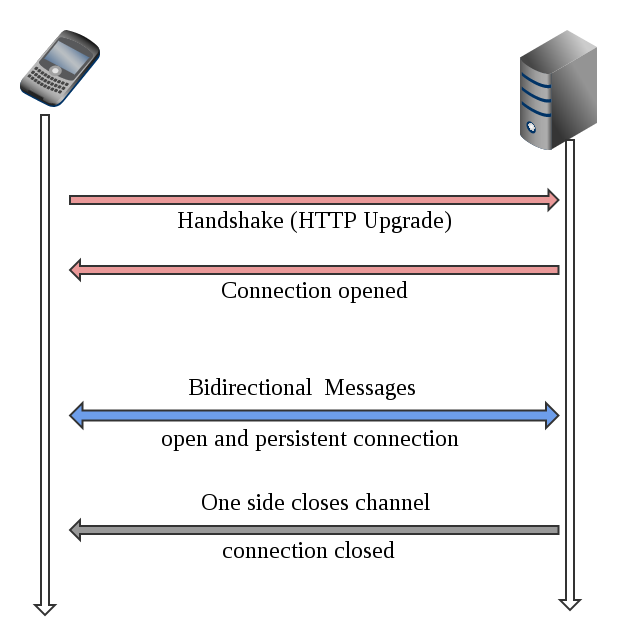
\includegraphics[scale=0.3]{websocket.png}
  \caption{Websocket handshake and communication}
\end{figure}

Another benefit to transporting data over HTTP is that many existing HTTP security mechanisms also apply to websocket.
With this unified security model, a list of standard HTTP security methods could be applied to a websocket connection.
For example, the same encryption as HTTPS using TLS/SSL. It's the same way to configure TLS encryption for websocket as you do for HTTPS with
certificates. In HTTPS, the client and server first establish a secure envelop which begin with HTTP protocol. Websocket Secure (WSS) use
the exactly the same way with handshake in HTTP, then upgrade to websocket protocol. 

\begin{figure}[tbph]
  \centering
  \label{fig:wss}
  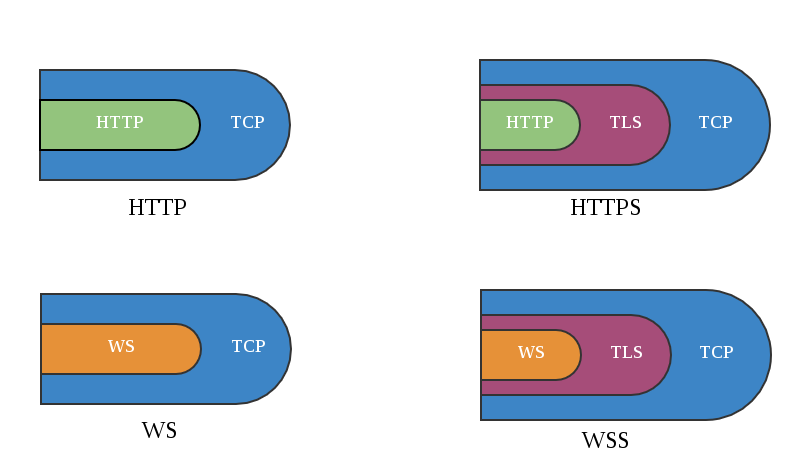
\includegraphics[scale=0.3]{wss.png}
  \caption{HTTPS and Websocket Secure}
\end{figure}

\subsection{HTTP Gateway} \label{HTTP Gateway}

One of the important concept of GNU Artanis is the HTTP Gateway. As mentioned earlier in this paper, HTTP Gateway is not a new concept,
for it's transparent in many server program.

The HTTP Gateway, as described intuitively, is a portal between client and customized protocol processing module of the server program,
and taking the HTTP negotiation to allow them to share information by communicating with the protocol over HTTP.

\begin{figure}[tbph]
  \centering
  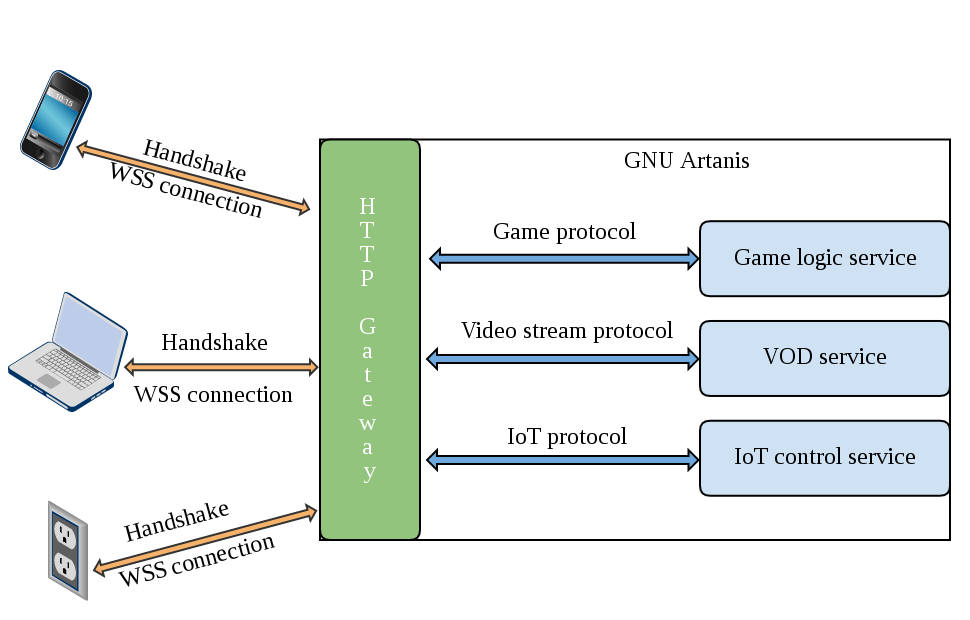
\includegraphics[scale=0.25]{httpgw.png}
  \caption{HTTP Gateway architecture in GNU Artanis}
  \label{fig:httpgw}
\end{figure}

The Figure \ref{fig:httpgw} shows the HTTP Gateway architecture in GNU Artanis.
It provides arbitrary protocol services over websockets. Beyond the web server, it becomes a {\it generic server}, which handles
connections of multi-protocols in the
same time. A {\it generic server} is rarely mentioned before, because most of the application of server programs are for dedicated protocol,
and to provide single service as its main duty.

For the {\it dedicated server}, FTP, HTTP as in web service, game server, IRC, etc. Usually, the remote server starts a service program
as a daemon listening on a TCP/UDP port according to a convention, and provides just one service in a dedicated protocol. Such a decoupled
pattern is obviously meets the KISS (Keep It Smart and Simple) principle. Moreover, when one service is down, it won't effect the others.

For the {\it generic server}, people don't have to listen on many TCP ports, there's just one port, 80 or 443 (for HTTPS). And the HTTP
Gateway will dispatch the requests to the related service, and maintain the long live session for each connection in a high concurrent way.
In the simplest way, all the services are running in GNU Artanis rather than standalone, and it's good for both quick developing and deployment.
Some people may think it's too tight coupled, if one of the services is broken, the whole GNU Artanis may down. How we solve it?
Fortunately, it is allowed to make each service standalone, similar to CGI, but in bytevector way according to websocket configuration, rather than HTTP requests redirecting. This would be good enough to solve the issue.

So, what's the value of a {\it generic server}?

It is obvious that the massive protocol-customized connections will appear in such a scenario like Internet of Things (IoT).
There'll be many IoT nodes as the massive clients, with many sensors or monitors, which may require many application level protocols,
although their messaging protocol maybe the same (MQTT over websocket).
For {\it generic server} reduces the workload of customizing and management of multi-protocols, and IoT based applications are
well-known to be the next big thing, the {\it generic server} may act important role in next decades. 

\subsection{Concurrency} \label{Concurrency}

The eternal subject of server side development is always concurrency.
Many years ago, the industry has been focusing on {\it C10K} problem dealing with at least $10,000$ connection concurrently.
Nowadays, it's becoming {\it C10M} which means at least 10 million connections concurrently.

No matter how the number is increasing, the main purpose is to hold more connections concurrently as possible.
Unfortunately, it is useless if one just purchase stronger machines with more RAM. In this way, the performance of single connection
processing could be higher, but increasing few connections concurrently.

The bottleneck is not the performance of machine, but the algorithm of events dispatching. The traditional select() and poll() are outdated,
for their $O(n)$ complexity drags the performance when it tries to query large number of sockets. The modern epoll() has
constant time complexity for that, say $O(1)$, and obviously win the title.

Beyond, the edge-trigger mode of epoll() co-operated with non-blocking I/O is widely used in the industry for high performance concurrent
programming.
It is believed that the concern of a server is not only about concurrency, but also the optimizing of the language implementation,
and better exception handling for robustness of the server system.

Of course, it's necessary to provide advanced scaling methodology for higher concurrency need to meet the future cloud computing. But it's
out of scope in this paper.

GNU Artanis choose epoll() for its I/O multiplexing, and take advantage of the non-blocking to implement asynchronous I/O in co-routines.
This model is proved to be practical and well-known in industry. We choose this model (epoll + non-blocking) to co-operate with co-routines
to provide good performance and concurrency.

\section{Some features in GNU Artanis} \label{Some features in GNU Artanis}

In addition to the server core, there're some notable features in GNU Artanis.

\subsection{RESTful}

REST stands for representational state transfer, which is an architectural style consisting of a coordinated set of components, connectors,
and data elements within a distributed hypermedia system, where the focus is on component roles and a specific set of interactions between data
elements rather than implementation details.

To the extent that systems conform to the constraints of REST they can be called RESTful. It is often communicate over HTTP with the same method
name (GET, POST, PUT, DELETE, etc.) that web browsers use to retrieve web pages and to send data to remote servers.
REST systems interface with external systems as web resources identified by URIs.

The name ``representational state'' is intended to evoke an image of how a well-designed Web application behaves: a network of web pages,
where the user progresses through the application by selecting links (state transitions), resulting in the next page (state) being transferred to
the user and rendered for their use.

\lstinputlisting{restful.scm}

\subsection{MVC}

Model-View-Controller (MVC) is a software architectural pattern for implementing user interfaces on computers. It divides a given software
application into three interconnected parts, so as to separate internal representations of information from the ways that information is
presented to or accepted from the user. Traditionally used for desktop graphical user interfaces (GUIs), this architecture has become extremely
popular for designing web applications.

The {\it Model} is the unchanging essence of the application/domain. And there'll be more than one interfaces with the {\it Model}, they're called
{\it Views}. The {\it Views} could be GUI, CLI or API. Although {\it Views} are very often graphical, they don’t have to be.
A {\it Controller} is an object that lets you manipulate a {\it View}. In a brief, {\it Controller} handles the input whilst the view handles the
output \citep{deacon2009model}.

GNU Artanis provides CLI tools for generating MVC template code, this will be introduced in \ref{CLI tools}.

\subsection{Relational Mapping}

Usually, Relational Mapping (RM) stands for ORM (Object Relational Mapping).
It is a programming technique for converting data between incompatible type systems in object-oriented (OO) programming languages.

However, although GNU Guile has an object system named GOOPS, GNU Artanis choose not to use OO for programming. It is enough
to use the features of Functional Programming (FP) to replace the essentials in OO, and it's proved in GNU Artanis development.
Because of this reason, GNU Artanis doesn't implement ORM, but closures to replace classes, and message passing for dispatching the methods
to mimic half-baked OO, which is more lightweight and less complexity than OO. It is called Functional Programming Relational Mapping (FPRM)
in GNU Artanis.

\subsection{Sessions}

HTTP sessions allows associating information with individual visitors.

A session is a semi-permanent interactive information interchange, also known as a dialogue, a conversation or a meeting, between two or more
communicating devices, or between a computer and user. A session is set up or established at a certain point in time, and then
torn down at some later point. An established communication session may involve more than one message in each direction. A session is typically,
but not always, stateful, meaning that at least one of the communicating parts needs to save information about the session history in order to be
able to communicate, as opposed to stateless communication, where the communication consists of independent requests with responses.

Traditionally, there're three kinds of session management in GNU Artanis:

\begin{itemize}
\item {\it Simple}, use hashtables for storing sessions in the memory;
\item {\it Filesystem}, use files for storing sessions;
\item {\it Database}, use Database for storing sessions.
\end{itemize}

\subsection{CLI tools} \label{CLI tools}

Providing CLI tools is becoming a fashion for most of the frameworks.
Basically, there're four commands in GNU Artanis:

To initialize a new application folder:
\begin{lstlisting}
  art create project-name
\end{lstlisting}

And the {\it draw} command is useful to generate MVC template code to save developers work:
\begin{lstlisting}
  art draw [controller/model] name
\end{lstlisting}
Note that {\it Views} are generated along with {\it Controllers}.

Sometimes it's necessary to move from one database vendor to another, or to upgrade the version of database software being used.
So the database migration could be useful to reconstruct the schema and tables, then import all the data to the new environment automatically.
\begin{lstlisting}
  art migrate operator name
\end{lstlisting}

The last but not least, the {\it work} command is used to start the server, and establish the service listening on the specified port.
\begin{lstlisting}
  art work
\end{lstlisting}

\section{Future work}

It is possible to implement map/reduce for cluster, and very high scalability with serializable continuations to scale the whole server
system by adding infinite nodes. These issues are open to be discussed and practiced in the future.

\acks

First, thanks free software movement and its community for all the contributions.

Thanks SZDIY community for providing all the conditions, and all the kindly encouraging. And I would like to thank my second daughter who
is only 18 days. It came suddenly in advanced that disorganized my writing plan. Fortunately, I have strong server core to handle these two
concurrent tasks, exhausted.


% We recommend abbrvnat bibliography style.

\bibliographystyle{unsrtabbrvnat}

% The bibliography should be embedded for final submission.
\softraggedright

\bibliography{mmrref}

\end{document}
